\chapter{Konzeption}
% TODO: weiter schreiben
Dieses Kapitel beinhaltet alle Schritte für die Konzeption der angewandte Methoden. Außerdem wird der Datensatz und die verwendete Frameworks 
präsentiert.

\section{Image Colorization als Multimodales Problem}
Konventionelle automatische Methoden zielen darauf ab, die Farben für ein generiertes Bild so nah wie möglich an das Originale Bild vorherzusagen.
Diese Methoden verwenden ein MSE Loss der Vorhersagen die Weit von den Originalen Farbwerte entfernt liegen, stärker bestraft, als Farbwerte
die dichter an den Originalen Farbwerte liegen. Das führt, wie bei \ref{subsection:verwandte-arbeiten} beschrieben, zu entsättigte Bilder.
Die Gründe für diese Ergebnisse ist dass verschiedene Objekte, verschiedene Farben einnehmen können. Aus diesem Grund, behandelt die vorliegende
Arbeit das Problem als ein Multimodales Problem.

% TODO: finish this
\section{Farbraum}
Der Standard Farbraum der Bilder für die Methoden dieser Arbeit ist der RGB-Farbraum. Bei diesem Farbraum lässt sich schwer das Graustufen Bild 
von den Farbkanäle zu trennen, daher wird der Lab-Farbraum verwendet.
\\
\\
Bei den Lab-Farbraum können ohne Probleme die Farbkanäle ``ab'' von den Belichtungskanal ``L'' getrennt werden. Der Belichtungskanal ``L'' 
enthält das Graustufenbild die in den CNN eingespeist wird. Das generierte Bild wird für die Darstellung von dem Lab-Farbraum in den RGB-Farbraum 
konvertiert.

\begin{figure}[H]
  \vspace{1cm}
  \begin{subfigure}
    \centering
    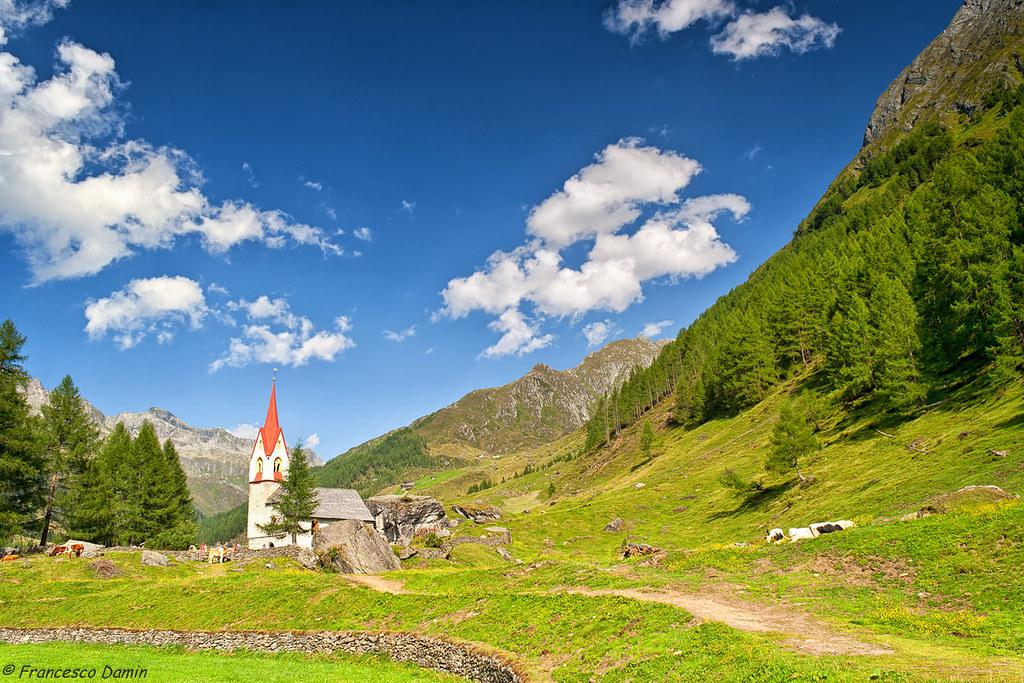
\includegraphics[width=.5\textwidth]{resources/colorspace/image.jpg}
  \end{subfigure}
  \begin{subfigure}
    \centering
    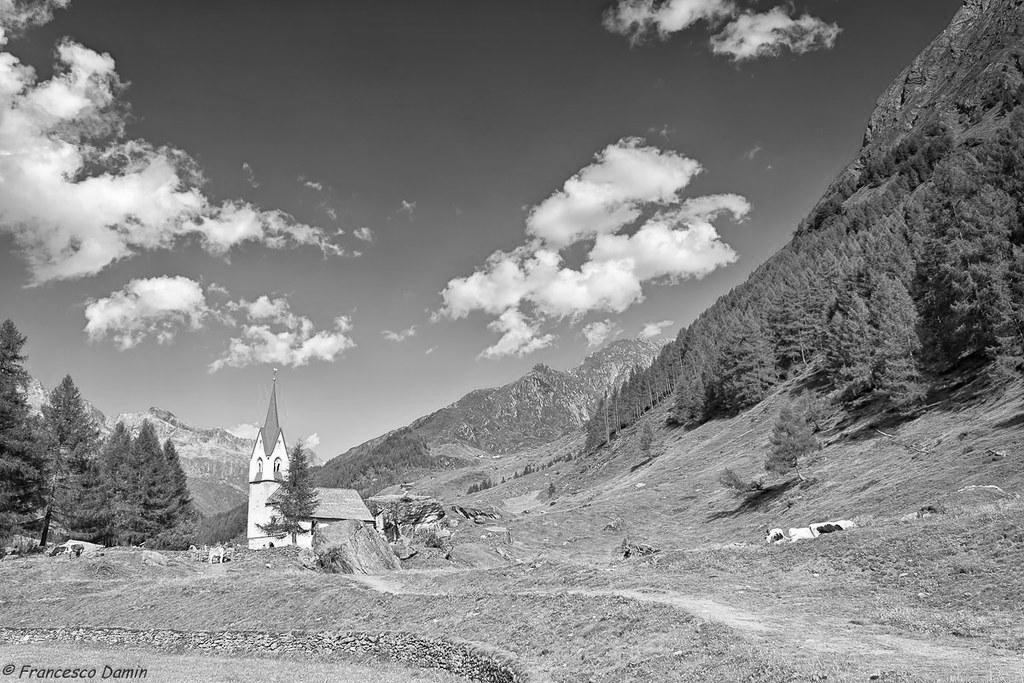
\includegraphics[width=.5\textwidth]{resources/colorspace/grayscale.png}
  \end{subfigure}
  \begin{subfigure}
    \centering
    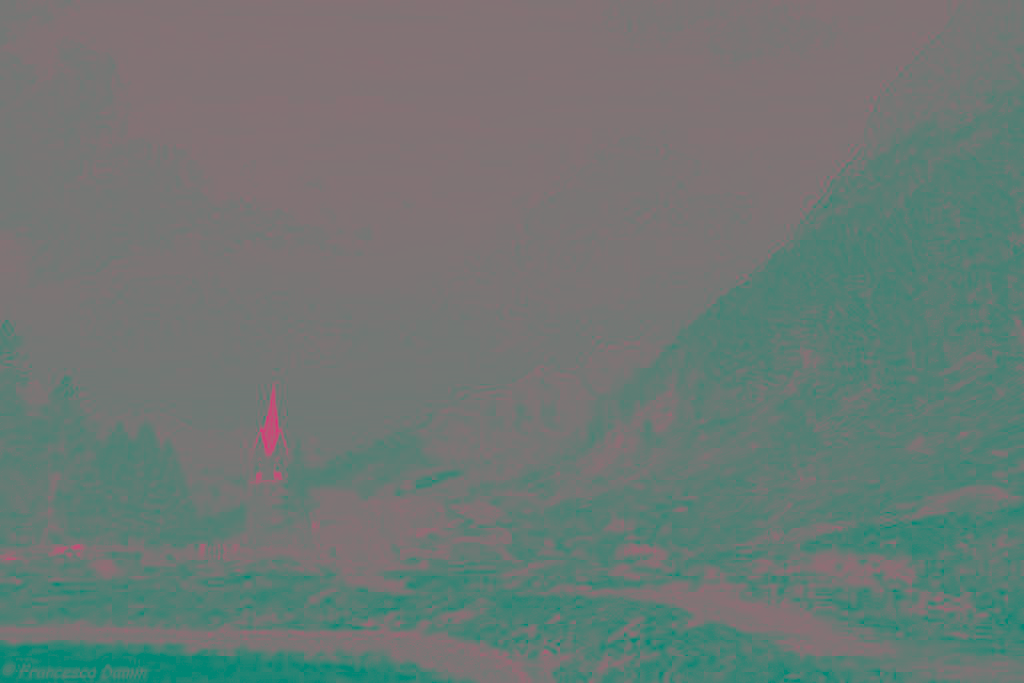
\includegraphics[width=.5\textwidth]{resources/colorspace/a_channel.png}
  \end{subfigure}
  \begin{subfigure}
    \centering
    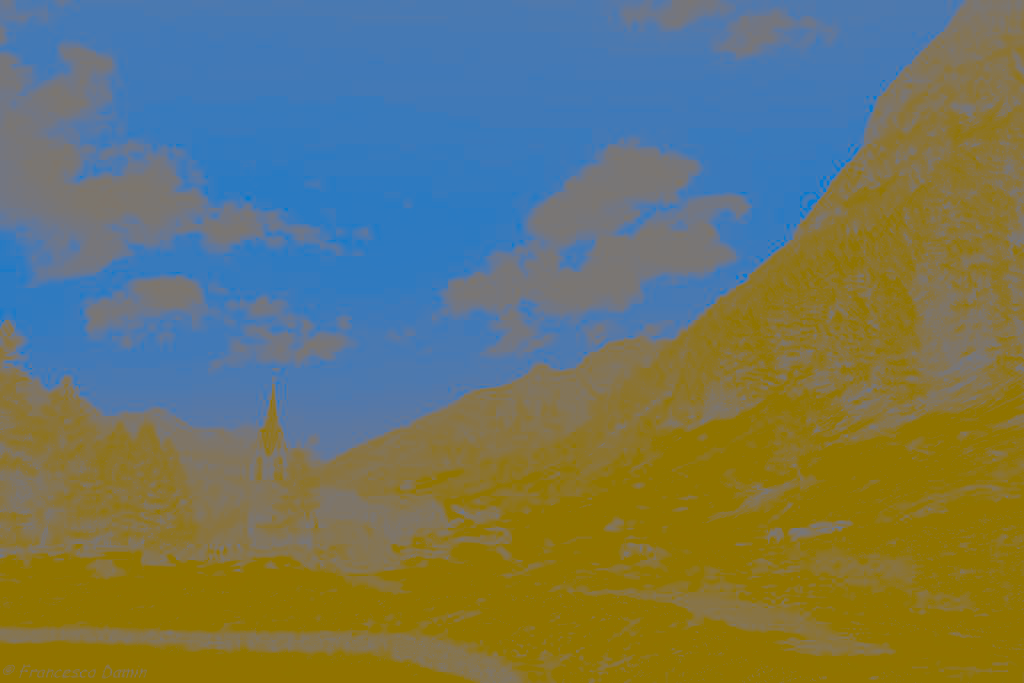
\includegraphics[width=.5\textwidth]{resources/colorspace/b_channel.png}
  \end{subfigure}
  \caption{Originales Bild oben links, den Belichtungskanal ``L'' oben rechts, unten links den Farbkanal ``a'' und unten rechts den Farbkanal ``b''.}
  \label{fig:fig}
\end{figure}

% TODO: maybe new image
\section{Binning}
Binning ist eine Technik, die für die Bildverarbeitung verwendet wird. Binning wird, in dem Kontext von Image Colorization, als Eingruppierung 
von naheliegenden Farben definiert. Die Farben werden in gleich große Intervalle aufgeteilt. Diese Intervalle bezeichnet man im Englischen als
``\gls{bin}s''. Jedes dieser Intervalle wird durch einen \gls{bin} Index repräsentiert, somit reduziert sich die Anzahl der Klassen die vorhergesagt werden
können.

Als Beispiel für die Veranschaulichung wird der normalisierte Lab-Farbraum in 36 gleich große \gls{bin}s unterteilt. Da die Farbinformationen 
in den ``ab'' Farbkanäle kodiert sind, werden nur diese 2 Farbkanäle in \gls{bin}s klassifiziert. Auf dem Bild \ref{image:bins} ist der Farbkanal 
``a'' auf der x-Achse und der ``b'' Farbkanal auf der y-Achse abgebildet. Die Vierecke repräsentieren die \gls{bin}s. Die obere Zahl in den Bins 
symbolisiert den Index auf dem \gls{grid}, die untere Zahl symbolisiert den Bin Index. Der Index auf den \gls{grid} ist Bedeutsam für die Berechnung der Bins.

\begin{figure}[H]
  \centering
  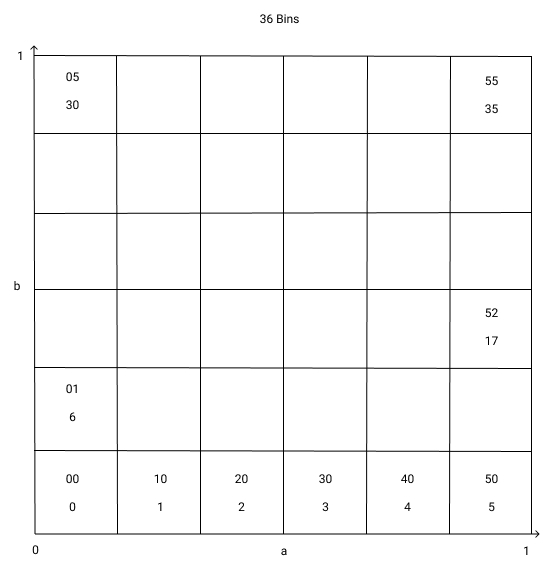
\includegraphics[width=0.55\textwidth]{resources/bins/bins.jpg}
  \caption{
  \gls{grid} mit 36 bins. Die x-Achse bildet die Werte von dem Farbkanal ``a'' und die y-Achse die Werte von den Farbkanal ``b'' ab.
  }
  \label{image:bins}
\end{figure}

Für die Methoden dieser Arbeit wurden nur symmetrische \gls{grid}s verwendet, so ergibt zum Beispiel ein $6 \times 6$ Grid 36 Bins und 
ein $18 \times 18$ Grid 324 Bins.

\section{Netzwerkarchitektur}
Die Netzwerkarchitektur ist ein wichtiger Faktor dass u.a. die Ergebnisse beeinträchtigen kann. Wichtig um die Methoden zu vergleichen ist ein
leichtes Netzwerk der wenige Parameter besitzt, schnell zu trainieren ist und gute Ergebnisse liefert.
\\
\\
Das Ziel von dem Netzwerk ist es, ein Graustufenbild als Input zu bekommen und eine Wahrscheinlichkeitsverteilung über alle Bins per Pixel vorherzusagen.
Das Output Volumen hat die Dimensionen $ W_{Input} \times H_{Input} \times 1 $, wobei $W$ und $H$ die Breite und Höhe von dem Bild sind,
mit einer Wahrscheinlichkeitsverteilung über alle Bins bei jedem Pixel. Dieser Ansatz ist auch bei Image Segmentation Probleme genutzt, wo ein Bild
in das Netzwerk einspeist wird und als Output, wird ein Segmentation map, mit eine Klasse per Pixel, erzeugt. In der Regel hat jeder Klasse eine
bestimmte Farbe und dadurch werden Objekte klassifiziert und getrennt. In dem Fall von Image Colorization bekommt jeder Pixel in dem Output Volumen
eine Wahrscheinlichkeitsverteilung über alle Bins die in einer Farbe umgewandelt wird.
\\
\\
Die Methoden von Zhang et al. \cite{zhang2016colorful} verwenden einen \gls{CNN} das einen Graustufenbild als Input entgegen nimmt und ein Volumen mit
eine Wahrscheinlichkeitsverteilung über alle Bins per Pixel generiert. Diese Netzwerkarchitektur besteht aus Blöcke mit jeweils 2 oder 3 Convolutional
und ReLU Layers, gefolgt von einem Batch Normalisation Layer. Batch Normalisation ist eine Regularisierungstechnik die die Werte in einem Hidden Layer
normalisiert, bevor sie in den nächsten Layer weitergereicht werden. Das Netzwerk hat keine Pooling Layers, alle Änderungen in der Auflösung werden durch
Downsampling oder Upsampling zwischen Blöcke erreicht.
\\
Dieser Netzwerkarchitektur ist sehr schwer für die GPU\footnote{Graphics Processing Unit}, was die Batch Größe und Trainingszeit stark beeinflusst.
\\
\\
Aus diesem Grund richtet sich die Netzwerkarchitektur dieser Arbeit nach der Netzwerkarchitektur von Billaut et al. \cite{billaut2018colorunet}. 
Sie verwenden eine angepasste Version von einem U-net Convolutional Neural Network \cite{ronneberger2015unet}. 

\subsection{U-net}
Ein U-net wird bei Image Segmentation angewendet und ist einer Art Autoencoder mit Skip Connections. Im vergleich zu konventionelle Autoencoder, können
der Encoder und Decoder nicht getrennt voneinander verwendet werden und bei dem Decoder werden Transposed Convolutions, als Upsampling 
Methode, verwendet. Das U-net verfügt außerdem über Skip Connections die ermöglichen fein-granuläre Details in dem Output Volumen zu 
wiederherstellen und helfen mit dem Vanishing Gradient Problem in Backpropagation. Skip Connections konkatenieren bestimmte Layers von dem
Encoder mit Layers von dem Decoder, mit der gleichen Dimensionen.
\\
\\
Ein U-net besteht, wie einem Autoencoder, aus einem Encoder und Decoder Teil. Der Encoder besteht aus sogenannten ``ConvBlocks''. ConvBlocks
bestehen aus 2 Convolutional Layers gefolgt von 2 Batch Normalisation Layers und ReLU als Aktivierungsfunktion. Die ConvBlocks werden gefolgt
von einem Pooling Layer die die Dimensionen von dem Volumen verringern. Der Decoder besteht aus ConvBlocks gefolgt von Transposed Convolutions
die die Dimensionen von dem Volumen wieder vergrößern. Das letzte Layer ist eine $1 \times 1$ Convolutional Layer die das Output Volumen generiert.
Skip Connections konkatenieren ConvBlocks aus dem Encoder mit den Transposed Convolutions aus dem Decoder, die die gleiche Dimensionen haben.

\begin{figure}[H]
  \centering
  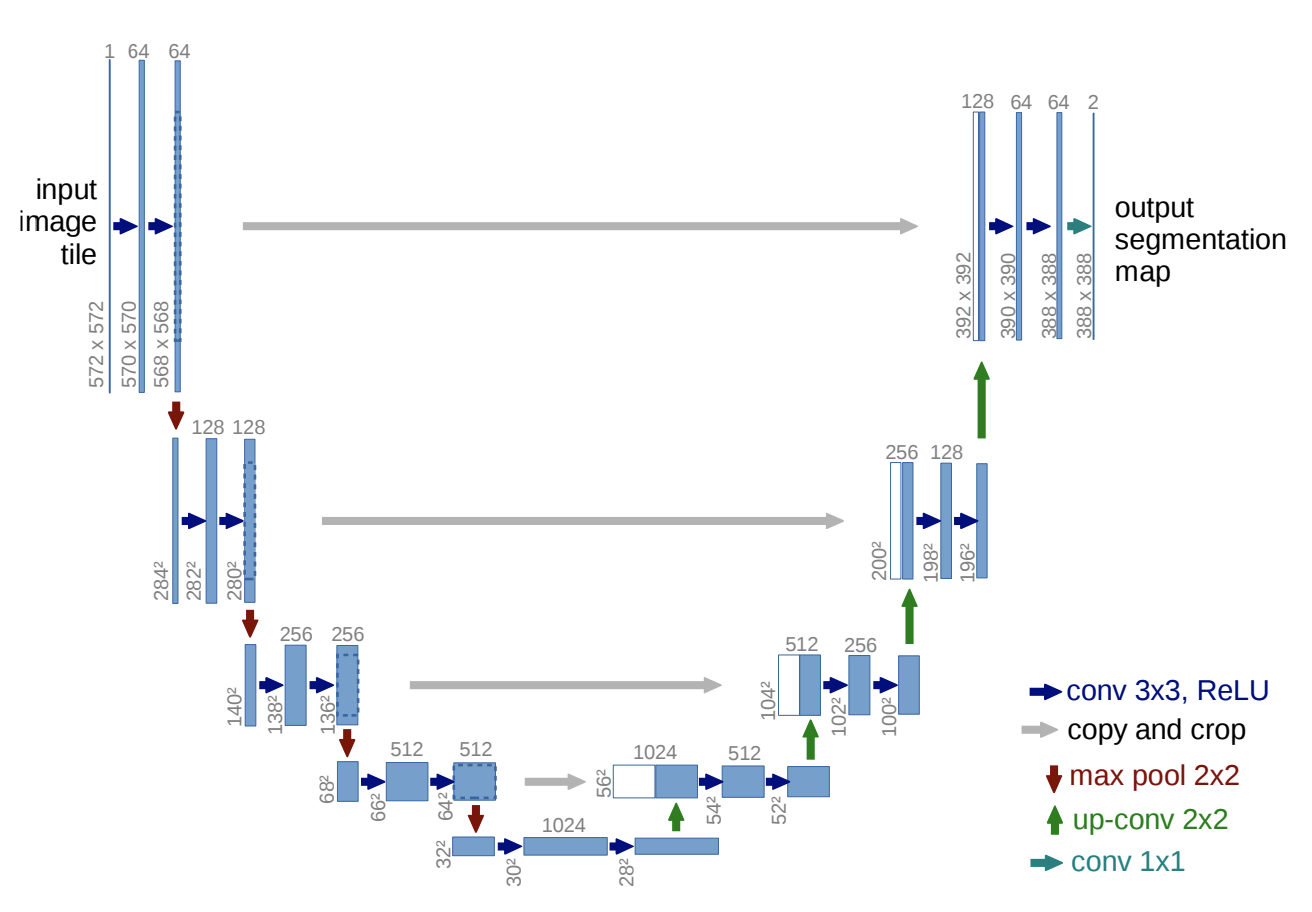
\includegraphics[width=0.75\textwidth]{resources/networks/unet.png}
  \caption{
    U-net Architektur
    \cite{ronneberger2015unet}
  }
  \label{image:unet}
\end{figure}


\section{Datensätze}
\section{Data Argumentation}
TODO
\section{Framework}